\section{Pianificazione}
\textit{TechSweave} ha deciso di pianificare il progetto in base alle scadenze sotto riportate. Di conseguenza il progetto è stato suddiviso nelle seguenti fasi:
\begin{itemize}
    \item Analisi;
    \item Consolidamento dei Requisiti;
    \item Progettazione architetturale;
    \item Progettazioni di dettaglio e codifica;
    \item Validazione e collaudo;
\end{itemize}
Ognuna di queste fasi verrà suddivisa in attività da realizzare entro i tempi stabiliti per la fase stessa e sarà mostrata nei rispettivi diagrammi di Gantt\textsubscript{\textbf{G}}.
\subsection{Analisi}
\textit{Periodo: dal 2021-03-11 al 2021-04-02}
Questo periodo corrisponde alla data di formazione del gruppo e termina con la data ultima per la consegna dei documenti relativi alla \textit{Revisione dei Requisiti}.\\
Questa fase è stata scomposta nelle seguenti attività che corrispondono ai documenti prodotti:
\begin{itemize}
    \item \textbf{Studio di Fattibilità:} viene effettuato uno studio dei capitolati comprendente i lati positivi e negativi a essi collegati, per poi selezionarne uno. L'attività è bloccante per l'\textit{Analisi dei Requisiti v2.0.0};
    \item \textbf{Norme di Progetto:} vengono specificate tutte le regole da rispettare durante lo sviluppo del progetto. Da questo documento dipenderanno le norme di stesura di tutti i prodotti successivi;
    \item \textbf{Analisi dei Requisiti:} vengono studiati e analizzati i requisiti legati al capitolato scelto nello \textit{Studio di Fattibilità v1.0.0};
    \item \textbf{Piano di Progetto:} il presente documento in cui attività, compiti e risorse precedentemente analizzate vengono distribuite tra i membri del team. Nel seguente documento è presente il calcolo del preventivo per la realizzazione del progetto;
    \item \textbf{Piano di Qualifica:} vengono individuati i metodi necessari per garantire la qualità del prodotto;
    \item \textbf{Glossario:} documento contenente tutti i termini che possono risultare ambigui durante lo svolgimento del progetto, di essi viene fornita una definizione sintetica ma esaustiva.
\end{itemize}
\begin{figure}[!ht]
    \caption{Diagramma di Gantt della fase di Analisi}
    \vspace{5px}
    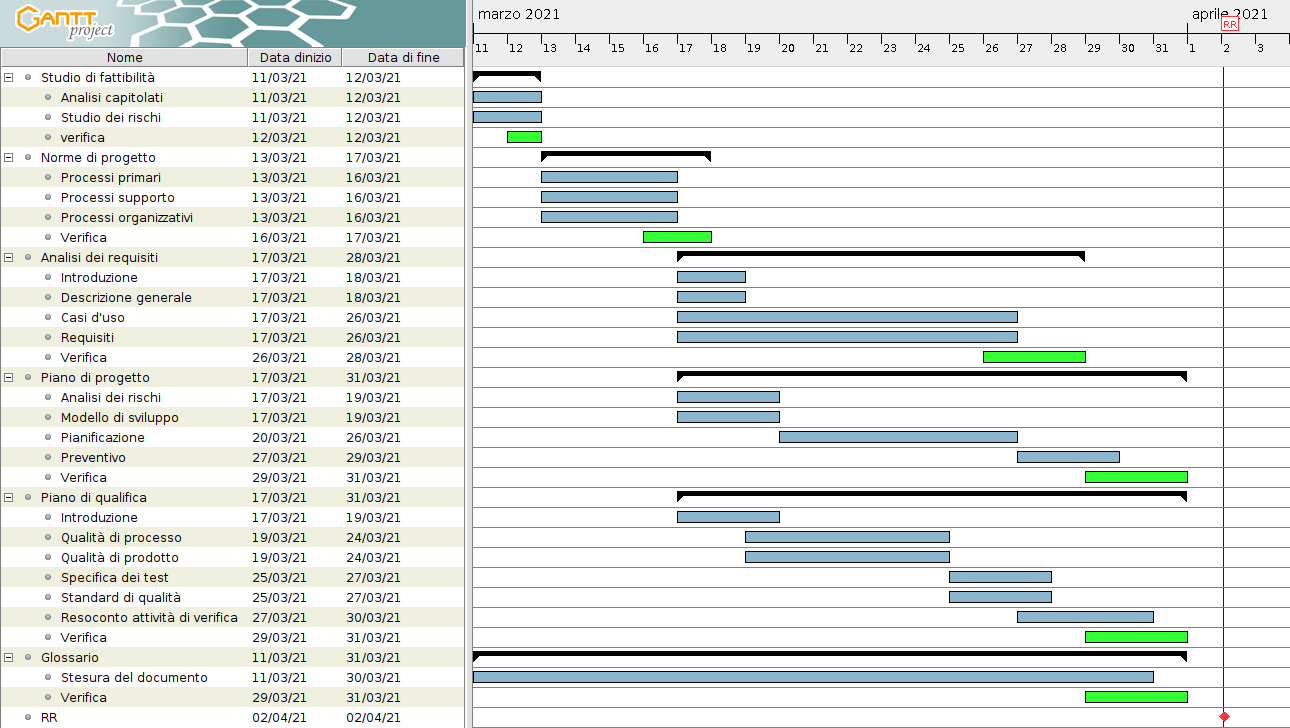
\includegraphics[scale=0.21]{../../../Images/Diagrammi/Gantt/diagramma_gantt_analisi_0.2.png}
    \centering
\end{figure}

\subsection{Consolidamento dei requisiti}
\textit{Periodo: dal 2021-04-02 al 2021-04-09}\\
Questa fase comincia con la fine di quella di Analisi e termina il giorno della presentazione della \textit{Revisione dei Requisiti}. Le attività di questa fase sono:
\begin{itemize}
    \item \textbf{Consolidamento:} con lo scopo di consolidare e migliorare i requisiti ottenuti nella fase precedente;
    \item \textbf{Preparazione alla presentazione:} per preparare il materiale necessario alla presentazione del 2021-04-09;
    \item \textbf{Incremento e Verifica:} nella quale vengono migliorati i documenti prodotti nella fase precedente se necessario;
    \item \textbf{Approfondimento personale:} ogni componente del gruppo dovrà dedicare delle ore di studio autonomo e approfondimento riguardo alle tecnologie necessarie per sviluppare il prodotto.
\end{itemize}
\begin{figure}[!ht]
    \caption{Diagramma di Gantt della fase di consolidamento dei requisiti}
    \vspace{5px}
    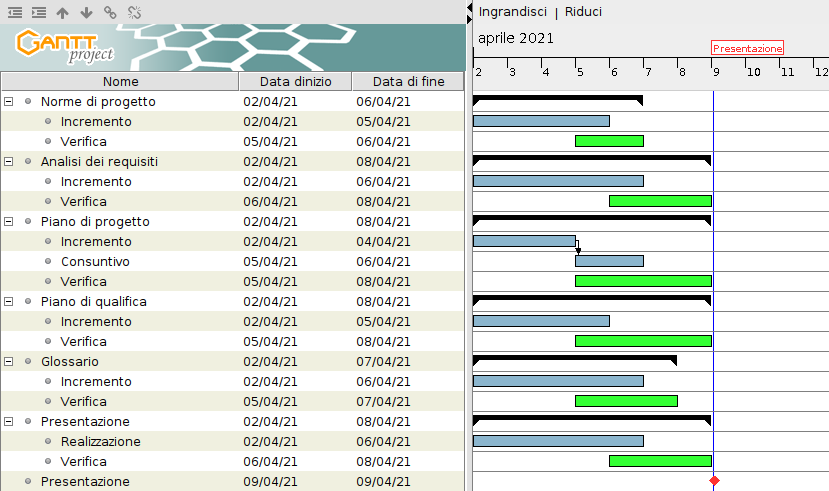
\includegraphics[scale=0.4]{../../../Images/Diagrammi/Gantt/consolidamento.png}
    \centering
\end{figure}
\pagebreak
\subsection{Progettazione architetturale}
\textit{Periodo: dal 2021-04-09 al 2021-05-03}\\
Questa fase comincia il giorno successivo alla presentazione e la sua fine coincide con la data di consegna della \textit{Revisione di Progettazione}. In questo lasso di tempo verrà individuata una soluzione architetturale che soddisfi i requisiti richiesti.\\
Le attività di questa fase sono:
\begin {itemize}
\item \textbf{Incremento e verifica:} in cui i documenti precedentemente redatti vengono aggiornati e migliorati;
\item \textbf{Technology Baseline\textsubscript{\textbf{G}}:} viene fatta un'analisi ad alto livello per comprendere appieno le tecnologie coinvolte, scegliendo l'architettura del codice e i design pattern\textsubscript{\textbf{G}} che saranno adoperati per lo sviluppo. Viene codificato il Proof of Concept\textsubscript{\textbf{G}} che sarà presentato o condiviso tramite repository con committente e proponente per verificare il corretto sviluppo del software.
\end {itemize}
\begin{figure}[!ht]
    \caption{Diagramma di Gantt dell'attività di progettazione architetturale}
    \vspace{5px}
    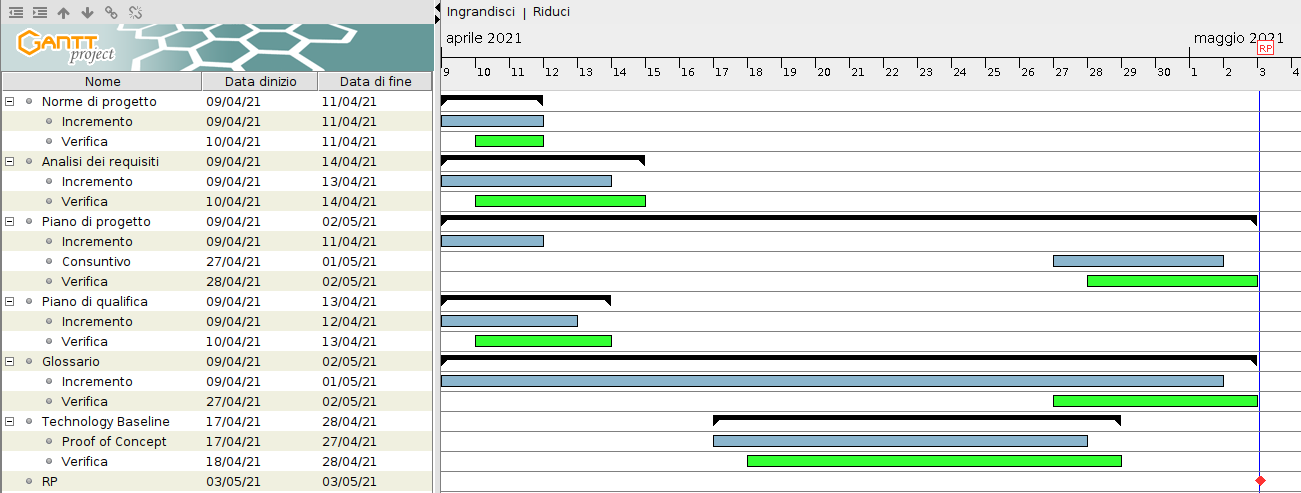
\includegraphics[scale=0.3]{../../../Images/Diagrammi/Gantt/progettArchitetturale_v2.png}
    \centering
\end{figure}

\subsection{Progettazione di dettaglio e codifica}
\textit{Periodo: dal 2021-05-10 al 2021-06-04}\\
L'inizio di questa fase è il giorno della scadenza della \textit{Revisione di Progettazione} e la data di fine coincide con la data di consegna dei documenti in vista della \textit{Revisione di Qualifica}.\\
Le attività di questa fase sono suddivisi in sette incrementi di sviluppo, per ognuno dei quali sono riportate le seguenti voci:
\begin{itemize}
    \item obbiettivi
          \begin{itemize}
              \item software;
              \item documentali;
          \end{itemize}
    \item periodo;
    \item ruoli attivi;
    \item attività previste;
    \item diagramma di Gantt.
\end{itemize}

%Incremento 1 RQ ---------------------------------------------------------
\subsubsection{Incremento 6}
\subsubsubsection{Obbiettivi}
Gli obbiettivi che il gruppo di pone di soddisfare in questo periodo sono i seguenti:
\begin{itemize}
    \item Preparazione alle attività di progettazione e codifica di dettaglio;
    \item Incremento della documentazione per verifica e miglioramento continuo.
\end{itemize}
\subsubsubsection{Periodo}
Il gruppo ritiene che per il raggiungimento degli obbiettivi serviranno quattro giorni di lavoro;\\
Il periodo interessato sarà dal 2021/05/10 al 2021/05/13
\subsubsubsection{Ruoli attivi}
Il gruppo ritiene che durante questo incremento saranno attivi i seguenti ruoli:
\begin{itemize}
    \item \textit{Responsabile di progetto};
    \item \textit{Amministratore di progetto};
    \item \textit{Progettista};
    \item \textit{Verificatore}.
\end{itemize}
\subsubsubsection{Attività previste}
Per soddisfare gli obbiettivi preposti il gruppo ritiene di dover svolgere le seguenti attività:
\begin{itemize}
    \item\textbf{integrazione strumenti:} integrazione degli strumenti necessari allo
          sviluppo del prodotto secondo gli standard qualitativi scelti;
    \item\textbf{analisi delle tecnologie:} studio delle tecnologie necessarie per lo sviluppo software;
    \item \textbf{verifica:} rilevazione delle metriche di qualità di prodotto e di processo;
    \item \textbf{ampliamento della documentazione:}
          \begin{itemize}
              \item estensione delle normative di progettazione e codifica;
              \item aggiornamento delle metriche e degli obbiettivi di qualità per quanto concerne il prodotto software;
              \item registrazione degli esiti di verifica;
              \item registrazione dell'andamento degli obbiettivi di qualità;
              \item aggiornamento dell'analisi dei rischi e della sua attualizzazione;
              \item aggiornamento del \textit{Glossario v3.0.0};
              \item calcolo del consuntivo di periodo;
              \item calcolo del preventivo a finire rispetto alla fase;
              \item calcolo del preventivo a finire rispetto al completamento del progetto.
          \end{itemize}
\end{itemize}

\subsubsubsection{Diagramma di Gantt}
\begin{figure}[!ht]
    \caption{Diagramma di Gantt dell'incremento 6}
    \vspace{5px}
    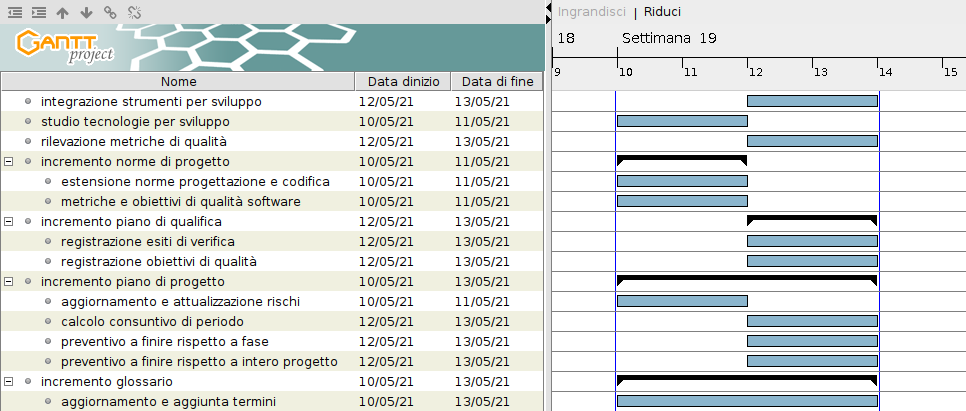
\includegraphics[scale=0.3]{../../../Images/Diagrammi/Gantt/incremento6.png}
    \centering
\end{figure}

%Incremento 2 RQ ---------------------------------------------------------
\subsubsection{Incremento 7}
\subsubsubsection{Obbiettivi}
Gli obbiettivi che il gruppo di pone di soddisfare in questo periodo sono i seguenti:
\begin{itemize}
    \item Miglioramento della struttura delle funzioni Lambda, con l'aggiunta dei filtri di ricerca;
    \item Miglioramento delle chiamate \textit{API GATEWAY} nel frontend per ottenere le informazioni delle funzioni lambda;
    \item Inizio della stesura della documentazione legata al prodotto software;
    \item Incremento della documentazione per verifica e miglioramento continuo.
\end{itemize}
\subsubsubsection{Periodo}
Il gruppo ritiene che per il raggiungimento degli obbiettivi serviranno quattro giorni di lavoro;\\
Il periodo interessato sarà dal 2021/05/14 al 2021/05/17
\subsubsubsection{Ruoli attivi}
Il gruppo ritiene che durante questo incremento saranno attivi i seguenti ruoli:
\begin{itemize}
    \item \textit{Responsabile di progetto};
    \item \textit{Amministratore di progetto};
    \item \textit{Progettista};
    \item \textit{Programmatore};
    \item \textit{Verificatore}.
\end{itemize}
\subsubsubsection{Attività previste}
Per soddisfare gli obbiettivi preposti il gruppo ritiene di dover svolgere le seguenti attività:
\begin{itemize}
    \item \textbf{codifica:}
          \begin{itemize}
              \item implementazione dei casi d'uso UC15- Scelta della categoria e UC35 - Applicazione dei filtri;\\ requisiti:
                    \begin{itemize}
                        \item R10F;                                                                   \item R10.1F
                        \item R10.2F;
                        \item R10.3F;
                        \item R10.5F;
                        \item R10.6F.
                    \end{itemize}
          \end{itemize}
    \item \textbf{pianificazione:} revisione della modalità di pianificazione gestendola attraverso gli incrementi;
    \item \textbf{progettazione di dettaglio:} inizio della stesura dell'\textit{Allegato Tecnico}:
          \begin{itemize}
              \item esposizione delle tecnologie;
              \item individuazione dei design pattern e della struttura del codice.
          \end{itemize}
    \item \textbf{verifica:} rilevazione delle metriche di qualità di prodotto e di processo;
    \item \textbf{ampliamento della documentazione:}
          \begin{itemize}
              \item inizio stesura \textit{Maintainer Manual v1.0.0} per le funzionalità complete;
              \item inizio stesura \textit{User Manual v1.0.0} per le funzionalità complete;
              \item registrazione degli esiti di verifica;
              \item registrazione dell'andamento degli obbiettivi di qualità;
              \item aggiornamento dell'analisi dei rischi e della sua attualizzazione;
              \item aggiornamento del \textit{Glossario v3.0.0};
              \item calcolo del consuntivo di periodo;
              \item calcolo del preventivo a finire rispetto alla fase;
              \item calcolo del preventivo a finire rispetto al completamento del progetto.
          \end{itemize}
\end{itemize}
\subsubsubsection{Diagramma di Gantt}
\begin{figure}[!ht]
    \caption{Diagramma di Gantt dell'incremento 7}
    \vspace{5px}
    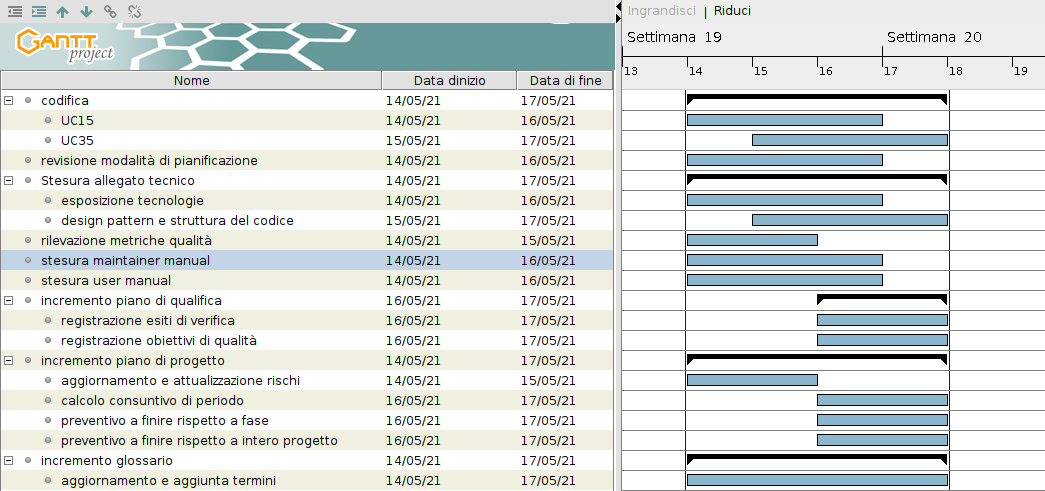
\includegraphics[scale=0.3]{../../../Images/Diagrammi/Gantt/incremento7.png}
    \centering
\end{figure}

%Incremento 3 RQ ---------------------------------------------------------
\subsubsection{Incremento 8}
\subsubsubsection{Obbiettivi}
Gli obbiettivi che il gruppo di pone di soddisfare in questo periodo sono i seguenti:
\begin{itemize}
    \item Ristrutturazione dei servizi lato backend;
    \item Riconfigurazione del linter \textit{eslint};
    \item Correzione della documentazione in base alla RP;
    \item Incremento della documentazione per verifica e miglioramento continuo.
\end{itemize}
\subsubsubsection{Periodo}
Il gruppo ritiene che per il raggiungimento degli obbiettivi serviranno tre giorni di lavoro;\\
Il periodo interessato sarà dal 2021/05/18 al 2021/05/20
\subsubsubsection{Ruoli attivi}
Il gruppo ritiene che durante questo incremento saranno attivi i seguenti ruoli:
\begin{itemize}
    \item \textit{Responsabile di progetto};
    \item \textit{Amministratore di progetto};
    \item \textit{Progettista};
    \item \textit{Programmatore};
    \item \textit{Verificatore}.
\end{itemize}
\subsubsubsection{Attività previste}
Per soddisfare gli obbiettivi preposti il gruppo ritiene di dover svolgere le seguenti attività:
\begin{itemize}
    \item \textbf{codifica:} ristrutturazione del codice per rispettare le indicazioni fornite dai proponenti;\\ requisiti:
          \begin{itemize}
              \item R8Q;
              \item R1v;
              \item R2v;
              \item R4v.
          \end{itemize}
    \item \textbf{configurazione linter:} riconfigurazione del linter \textit{eslint} rispettando le indicazioni fornite dai proponenti. Aggiunta del linter ai sistemi di \textit{continuous integration};
    \item \textbf{progettazione di dettaglio}: incremento della stesura dell'\textit{Allegato Tecnico}:
          \begin{itemize}
              \item aggiunta dei diagrammi delle classi;
              \item aggiunta dei diagrammi di sequenza.
          \end{itemize}
    \item \textbf{verifica:} rilevazione delle metriche di qualità di prodotto e di processo;
    \item \textbf{ampliamento della documentazione:}
          \begin{itemize}
              \item incremento della stesura del \textit{Maintainer Manual v1.0.0} per le funzionalità complete;
              \item incremento della stesura del \textit{User Manual v1.0.0} per le funzionalità complete;
              \item registrazione degli esiti di verifica;
              \item registrazione dell'andamento degli obbiettivi di qualità;
              \item aggiornamento dell'analisi dei rischi e della sua attualizzazione;
              \item aggiornamento del \textit{Glossario v3.0.0};
              \item calcolo del consuntivo di periodo;
              \item calcolo del preventivo a finire rispetto alla fase;
              \item calcolo del preventivo a finire rispetto al completamento del progetto.
          \end{itemize}
\end{itemize}
\subsubsubsection{Diagramma di Gantt}
\begin{figure}[!ht]
    \caption{Diagramma di Gantt dell'incremento 8}
    \vspace{5px}
    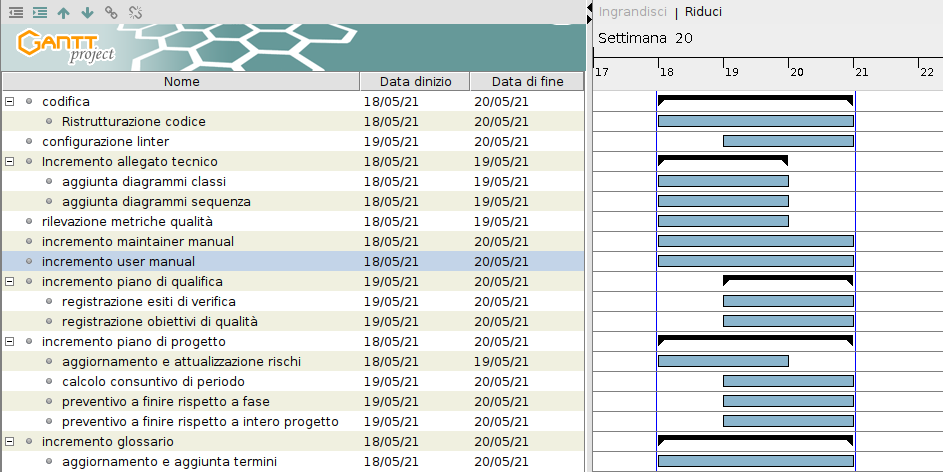
\includegraphics[scale=0.3]{../../../Images/Diagrammi/Gantt/incremento8.png}
    \centering
\end{figure}

%Incremento 4 RQ ---------------------------------------------------------
\subsubsection{Incremento 9}
\subsubsubsection{Obbiettivi}
Gli obbiettivi che il gruppo di pone di soddisfare in questo periodo sono i seguenti:
\begin{itemize}
    \item Distinzione tra cliente e venditore;
    \item Implementazione lato frontend;
    \item Incremento della documentazione per verifica e miglioramento continuo.
\end{itemize}
\subsubsubsection{Periodo}
Il gruppo ritiene che per il raggiungimento degli obbiettivi serviranno due giorni di lavoro;\\
Il periodo interessato sarà dal 2021/05/21 al 2021/05/22
\subsubsubsection{Ruoli attivi}
Il gruppo ritiene che durante questo incremento saranno attivi i seguenti ruoli:
\begin{itemize}
    \item \textit{Responsabile di progetto};
    \item \textit{Amministratore di progetto};
    \item \textit{Progettista};
    \item \textit{Programmatore};
    \item \textit{Verificatore}.
\end{itemize}
\subsubsubsection{Attività previste}
Per soddisfare gli obbiettivi preposti il gruppo ritiene di dover svolgere le seguenti attività:
\begin{itemize}
    \item \textbf{codifica:}
          \begin{itemize}
              \item implementazione del caso d'uso UC17 - Gestione profilo;\\
                    requisiti:
                    \begin{itemize}
                        \item R15F;
                        \item R15.1F;
                        \item R15.2F;
                        \item R15.3F.
                    \end{itemize}
              \item implementazione del caso d'uso UC19 - Visualizzazione profilo;\\
                    requisiti:
                    \begin{itemize}
                        \item R17F.
                    \end{itemize}
              \item implementazione del caso d'uso UC37 - Modifica della password;\\
                    requisiti:
                    \begin{itemize}
                        \item R32F.
                    \end{itemize}
          \end{itemize}
    \item \textbf{progettazione di dettaglio}: incremento della stesura dell'\textit{Allegato Tecnico}:
          \begin{itemize}
              \item aggiunta dei diagrammi di attività.
          \end{itemize}
    \item \textbf{verifica:} rilevazione delle metriche di qualità di prodotto e di processo;
    \item \textbf{ampliamento della documentazione:}
          \begin{itemize}
              \item incremento della stesura del \textit{Maintainer Manual v1.0.0} per le funzionalità complete;
              \item incremento della stesura del \textit{User Manual v1.0.0} per le funzionalità complete;
              \item registrazione degli esiti di verifica;
              \item registrazione dell'andamento degli obbiettivi di qualità;
              \item aggiornamento dell'analisi dei rischi e della sua attualizzazione;
              \item aggiornamento del \textit{Glossario v3.0.0};
              \item calcolo del consuntivo di periodo;
              \item calcolo del preventivo a finire rispetto alla fase;
              \item calcolo del preventivo a finire rispetto al completamento del progetto.
          \end{itemize}
\end{itemize}
\pagebreak
\subsubsubsection{Diagramma di Gantt}
\begin{figure}[!ht]
    \caption{Diagramma di Gantt dell'incremento 9}
    \vspace{5px}
    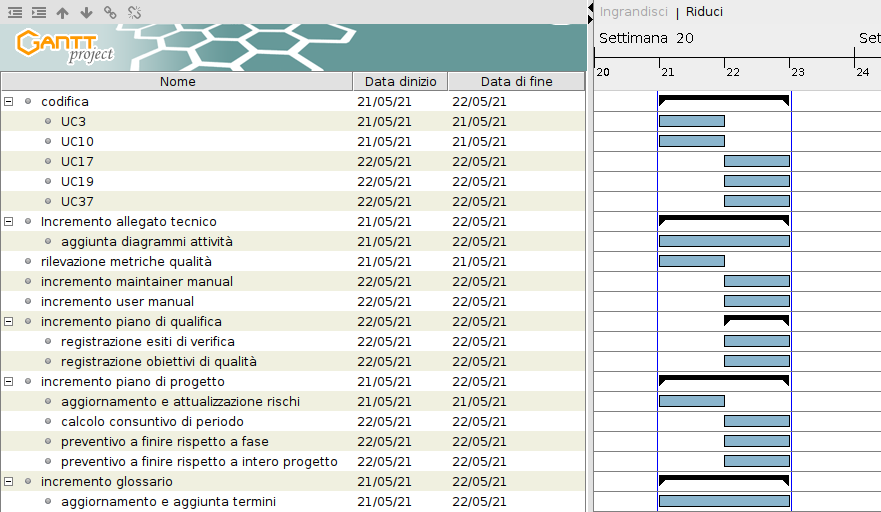
\includegraphics[scale=0.3]{../../../Images/Diagrammi/Gantt/incremento9.png}
    \centering
\end{figure}

%Incremento 5 RQ ---------------------------------------------------------
\subsubsection{Incremento 10}
\subsubsubsection{Obbiettivi}
Gli obbiettivi che il gruppo di pone di soddisfare in questo periodo sono i seguenti:
\begin{itemize}
    \item Completamento Checkout;
    \item Completamento carrello;
    \item Completamento pagina PDP;
    \item Incremento della documentazione per verifica e miglioramento continuo.
\end{itemize}
\subsubsubsection{Periodo}
Il gruppo ritiene che per il raggiungimento degli obbiettivi serviranno tre giorni di lavoro;\\
Il periodo interessato sarà dal 2021/05/23 al 2021/05/25
\subsubsubsection{Ruoli attivi}
Il gruppo ritiene che durante questo incremento saranno attivi i seguenti ruoli:
\begin{itemize}
    \item \textit{Responsabile di progetto};
    \item \textit{Amministratore di progetto};
    \item \textit{Progettista};
    \item \textit{Programmatore};
    \item \textit{Verificatore}.
\end{itemize}
\subsubsubsection{Attività previste}
Per soddisfare gli obbiettivi preposti il gruppo ritiene di dover svolgere le seguenti attività:
\begin{itemize}
    \item \textbf{codifica:}
          \begin{itemize}
              \item implementazione del caso d'uso UC4 - Visualizzazione dettagli di un prodotto;\\
                    requisiti:
                    \begin{itemize}
                        \item R5F;
                        \item R5.8F.
                    \end{itemize}
              \item implementazione del caso d'uso UC5 - Aggiunta di un prodotto al carrello;\\
                    requisiti:
                    \begin{itemize}
                        \item R6F.
                    \end{itemize}
              \item implementazione del caso d'uso UC11 - Visualizzazione dei prodotti inseriti nel carrello;\\
                    requisiti:
                    \begin{itemize}
                        \item R13.5F.
                    \end{itemize}
              \item implementazione del caso d'uso UC12 - Rimozione di un prodotto dal carrello;\\
                    requisiti:
                    \begin{itemize}
                        \item R13.2F.
                    \end{itemize}
              \item implementazione del caso d'uso UC13 - Modifica della quantità di un prodotto nel carrello;\\
                    requisiti:
                    \begin{itemize}
                        \item R13.3F.
                    \end{itemize}
              \item implementazione del caso d'uso UC14 - Visualizzazione errore quantità superata di un prodotto nel carrello;\\
                    requisiti:
                    \begin{itemize}
                        \item R13.3F.
                    \end{itemize}
              \item implementazione del caso d'uso UC21 - Checkout;\\
                    requisiti:
                    \begin{itemize}
                        \item R19F;
                        \item R19.1F;
                        \item R19.2F;
                        \item R19.3F.
                    \end{itemize}
              \item implementazione del caso d'uso UC22 -  Annullamento checkout;\\
                    requisiti:
                    \begin{itemize}
                        \item R20F.
                    \end{itemize}
              \item implementazione del caso d'uso UC23 -  Riepilogo ordine;\\
                    requisiti:
                    \begin{itemize}
                        \item R21F.
                    \end{itemize}
              \item implementazione del caso d'uso UC24 - Visualizzazione degli ordini effettuati;\\
                    requisiti:
                    \begin{itemize}
                        \item R22F.
                    \end{itemize}
              \item implementazione del caso d'uso UC36 -  Errore nel pagamento;\\
                    requisiti:
                    \begin{itemize}
                        \item R19.4F.
                    \end{itemize}
          \end{itemize}
    \item \textbf{verifica:} rilevazione delle metriche di qualità di prodotto e di processo;
    \item \textbf{ampliamento della documentazione:}
          \begin{itemize}
              \item incremento della stesura del \textit{Maintainer Manual v1.0.0} per le funzionalità complete;
              \item incremento della stesura del \textit{User Manual v1.0.0} per le funzionalità complete;
              \item registrazione degli esiti di verifica;
              \item registrazione dell'andamento degli obbiettivi di qualità;
              \item aggiornamento dell'analisi dei rischi e della sua attualizzazione;
              \item aggiornamento del \textit{Glossario v3.0.0};
              \item calcolo del consuntivo di periodo;
              \item calcolo del preventivo a finire rispetto alla fase;
              \item calcolo del preventivo a finire rispetto al completamento del progetto.
          \end{itemize}
\end{itemize}
\subsubsubsection{Diagramma di Gantt}
\begin{figure}[!ht]
    \caption{Diagramma di Gantt dell'incremento 10}
    \vspace{5px}
    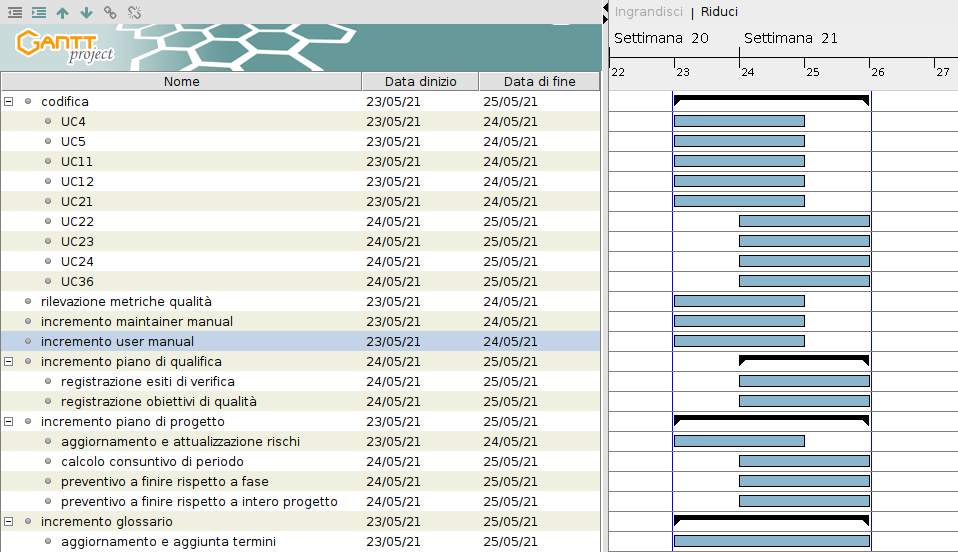
\includegraphics[scale=0.3]{../../../Images/Diagrammi/Gantt/incremento10.png}
    \centering
\end{figure}

%Incremento 6 RQ ---------------------------------------------------------
\subsubsection{Incremento 11}
\subsubsubsection{Obbiettivi}
Gli obbiettivi che il gruppo di pone di soddisfare in questo periodo sono i seguenti:
\begin{itemize}
    \item Completamento Homepage;
    \item Completamento PLP;
    \item Implementazione ricerca di un prodotto;
    \item Incremento della documentazione per verifica e miglioramento continuo.
\end{itemize}
\subsubsubsection{Periodo}
Il gruppo ritiene che per il raggiungimento degli obbiettivi serviranno due giorni di lavoro;\\
Il periodo interessato sarà dal 2021/05/26 al 2021/05/27
\subsubsubsection{Ruoli attivi}
Il gruppo ritiene che durante questo incremento saranno attivi i seguenti ruoli:
\begin{itemize}
    \item \textit{Responsabile di progetto};
    \item \textit{Amministratore di progetto};
    \item \textit{Programmatore};
    \item \textit{Verificatore}.
\end{itemize}
\subsubsubsection{Attività previste}
Per soddisfare gli obbiettivi preposti il gruppo ritiene di dover svolgere le seguenti attività:
\begin{itemize}
    \item \textbf{codifica:}
          \begin{itemize}
              \item completamento implementazione homepage;\\ requisiti:
                    \begin{itemize}
                        \item R1.1F;
                        \item R10.1F;
                        \item R1.2F.
                    \end{itemize}
              \item implementazione dei casi d'uso UC6 - Ricerca dei prodotti;\\ requisiti:
                    \begin{itemize}
                        \item R7F.
                    \end{itemize}
              \item implementazione dei casi d'uso UC7 - Visualizzazione della lista dei prodotti;\\ requisiti:
                    \begin{itemize}
                        \item R8F.
                    \end{itemize}
          \end{itemize}
    \item \textbf{verifica:} rilevazione delle metriche di qualità di prodotto e di processo;
    \item \textbf{ampliamento della documentazione:}
          \begin{itemize}
              \item registrazione degli esiti di verifica;
              \item registrazione dell'andamento degli obbiettivi di qualità;
              \item aggiornamento dell'analisi dei rischi e della sua attualizzazione;
              \item aggiornamento del \textit{Glossario v3.0.0};
              \item calcolo del consuntivo di periodo;
              \item calcolo del preventivo a finire rispetto alla fase;
              \item calcolo del preventivo a finire rispetto al completamento del progetto.
          \end{itemize}
\end{itemize}

\subsubsubsection{Diagramma di Gantt}
\begin{figure}[!ht]
    \caption{Diagramma di Gantt dell'incremento 11}
    \vspace{5px}
    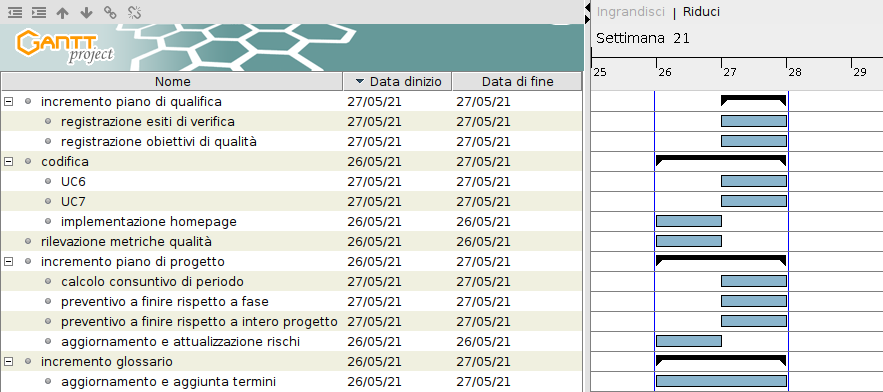
\includegraphics[scale=0.3]{../../../Images/Diagrammi/Gantt/incremento11.png}
    \centering
\end{figure}

%Incremento 7 RQ ---------------------------------------------------------
\subsubsection{Incremento 12}
\subsubsubsection{Obbiettivi}
\begin{itemize}
    \item Completamento pagina venditore;
    \item Aggiunta sezione per la gestione delle categorie;
    \item Aggiunta visualizzazione elenco clienti e ordini ricevuti;
    \item Aggiunta sezione per la gestione di un prodotto;
    \item Incremento della documentazione per verifica e miglioramento continuo.
\end{itemize}
Gli obbiettivi che il gruppo di pone di soddisfare in questo periodo sono i seguenti:
\subsubsubsection{Periodo}
Il gruppo ritiene che per il raggiungimento degli obbiettivi serviranno tre giorni di lavoro;\\
Il periodo interessato sarà dal 2021/05/28 al 2021/05/30
\subsubsubsection{Ruoli attivi}
Il gruppo ritiene che durante questo incremento saranno attivi i seguenti ruoli:
\begin{itemize}
    \item \textit{Responsabile di progetto};
    \item \textit{Amministratore di progetto};
    \item \textit{Programmatore};
    \item \textit{Verificatore}.
\end{itemize}
\subsubsubsection{Attività previste}
Per soddisfare gli obbiettivi preposti il gruppo ritiene di dover svolgere le seguenti attività:
\begin{itemize}
    \item \textbf{codifica:}
          \begin{itemize}
              \item implementazione del caso d'uso UC25 - Visualizzazione della lista dei clienti;\\
                    requisiti:
                    \begin{itemize}
                        \item R23F.
                    \end{itemize}
              \item implementazione del caso d'uso UC26 - Visualizzazione della lista degli ordini;\\
                    requisiti:
                    \begin{itemize}
                        \item R24F.
                    \end{itemize}
              \item implementazione del caso d'uso UC28 -  Aggiunta di un prodotto;\\
                    requisiti:
                    \begin{itemize}
                        \item R26F.
                    \end{itemize}
              \item implementazione del caso d'uso UC29 - Modifica di un prodotto;\\
                    requisiti:
                    \begin{itemize}
                        \item R27F.
                    \end{itemize}
              \item implementazione del caso d'uso UC30 - Rimozione di un prodotto;\\
                    requisiti:
                    \begin{itemize}
                        \item R28F.
                    \end{itemize}
              \item implementazione del caso d'uso UC31 -  Aggiunta di una categoria;\\
                    requisiti:
                    \begin{itemize}
                        \item R29F.
                    \end{itemize}
              \item implementazione del caso d'uso UC32 -  Rimozione di una categoria;\\
                    requisiti:
                    \begin{itemize}
                        \item R30F.
                    \end{itemize}
          \end{itemize}
    \item \textbf{verifica:} rilevazione delle metriche di qualità di prodotto e di processo;
    \item \textbf{ampliamento della documentazione:}
          \begin{itemize}
              \item registrazione degli esiti di verifica;
              \item registrazione dell'andamento degli obbiettivi di qualità;
              \item aggiornamento dell'analisi dei rischi e della sua attualizzazione;
              \item aggiornamento del \textit{Glossario v3.0.0};
              \item calcolo del consuntivo di periodo;
              \item calcolo del preventivo a finire rispetto alla fase;
              \item calcolo del preventivo a finire rispetto al completamento del progetto.
          \end{itemize}
\end{itemize}
\subsubsubsection{Diagramma di Gantt}
\begin{figure}[!ht]
    \caption{Diagramma di Gantt dell'incremento 12}
    \vspace{5px}
    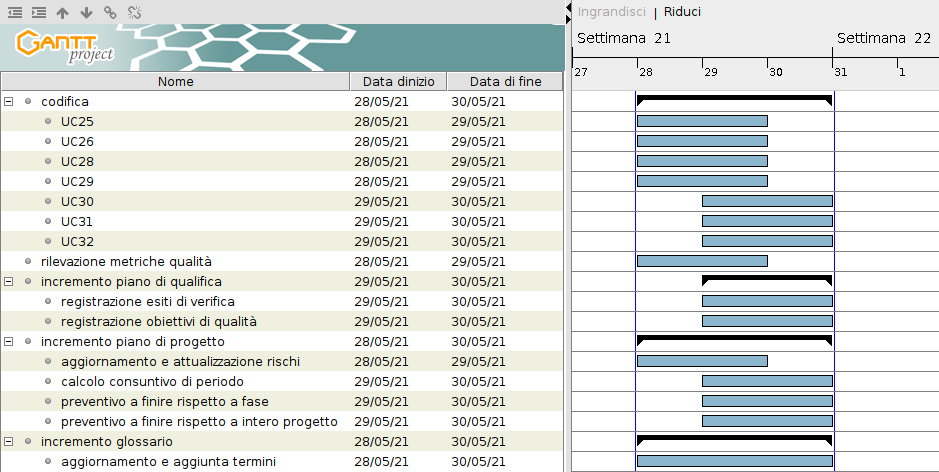
\includegraphics[scale=0.3]{../../../Images/Diagrammi/Gantt/incremento12.png}
    \centering
\end{figure}

%Incremento 8 RQ ---------------------------------------------------------
\subsubsection{Incremento 13}
\subsubsubsection{Obbiettivi}
Gli obbiettivi che il gruppo di pone di soddisfare in questo periodo sono i seguenti:
\begin{itemize}
    \item Preparazione per la \textit{Revisione di Qualifica};
    \item Correzione del codice secondo le indicazioni ricevute durante la \textit{Product Baseline} e con il proponente;
    \item Correzione dell'\textbf{Allegato Tecnico};
    \item Incremento della documentazione per verifica e miglioramento continuo.
\end{itemize}
\subsubsubsection{Periodo}
Il gruppo ritiene che per il raggiungimento degli obbiettivi serviranno quattro giorni di lavoro;\\
Il periodo interessato sarà dal 2021/05/31 al 2021/06/03
\subsubsubsection{Ruoli attivi}
Il gruppo ritiene che durante questo incremento saranno attivi i seguenti ruoli:
\begin{itemize}
    \item \textit{Responsabile di progetto};
    \item \textit{Amministratore di progetto};
    \item \textit{Programmatore};
    \item \textit{Verificatore}.
\end{itemize}
\subsubsubsection{Attività previste}
Per soddisfare gli obbiettivi preposti il gruppo ritiene di dover svolgere le seguenti attività:
\begin{itemize}
    \item\textbf{codifica:}
    \item \begin{itemize}
              \item correzione in base alle indicazioni ricevute durante la \textit{Product Baseline};
              \item correzione in base alle indicazioni ricevute dal proponente.
          \end{itemize}
    \item \textbf{verifica:} rilevazione delle metriche di qualità di prodotto e di processo;
    \item \textbf{ampliamento della documentazione:}
          \begin{itemize}
              \item registrazione degli esiti di verifica;
              \item registrazione dell'andamento degli obbiettivi di qualità;
              \item aggiornamento dell'analisi dei rischi e della sua attualizzazione;
              \item aggiornamento del \textit{Glossario v3.0.0};
              \item calcolo del consuntivo di periodo;
              \item calcolo del preventivo a finire rispetto alla fase;
              \item calcolo del preventivo a finire rispetto al completamento del progetto.
          \end{itemize}
\end{itemize}
\subsubsubsection{Diagramma di Gantt}
\begin{figure}[!ht]
    \caption{Diagramma di Gantt dell'incremento 13}
    \vspace{5px}
    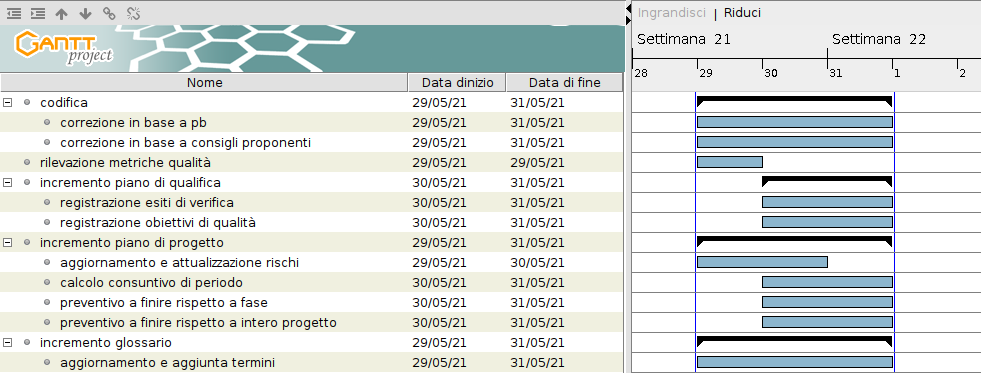
\includegraphics[scale=0.3]{../../../Images/Diagrammi/Gantt/incremento13.png}
    \centering
\end{figure}

% \begin{itemize}
%     \item \textbf{Incremento e verifica:} in cui i documenti precedentemente redatti vengono aggiornati e migliorati;
%     \item \textbf{Product Baseline\textsubscript{\textbf{G}}}: a seguito della \textit{Technology Baseline} l'architettura individuata in essa viene scomposta nelle sue unità, che vengono analizzate in profondità per fornire i dettagli necessari alla loro codifica e verifica;
%     \item \textbf{Codifica:} questa attività consiste nella scrittura e verifica del codice secondo i modi definiti nel \textit{Piano di Qualifica v2.0.0}.
%     \item \textbf{Specifica Tecnica:} Viene redatto un documento contenente tutte le caratteristiche del prodotto e le motivazioni che hanno portato alla loro scelta;
%     \item \textbf{User Manual:} viene redatto un documento contenente le istruzioni d'uso del software da parte dell'utente.
% \end{itemize}
\subsubsection{Diagramma di Gantt della fase}
In base alle attività pianificate negli incrementi e alla loro distribuzione nel tempo, la pianificazione complessiva della fase può essere riassunta nel seguente diagramma.
\begin{figure}[!ht]
    \caption{Diagramma di Gantt dell'attività di progettazione di dettaglio e codifica}
    \vspace{5px}
    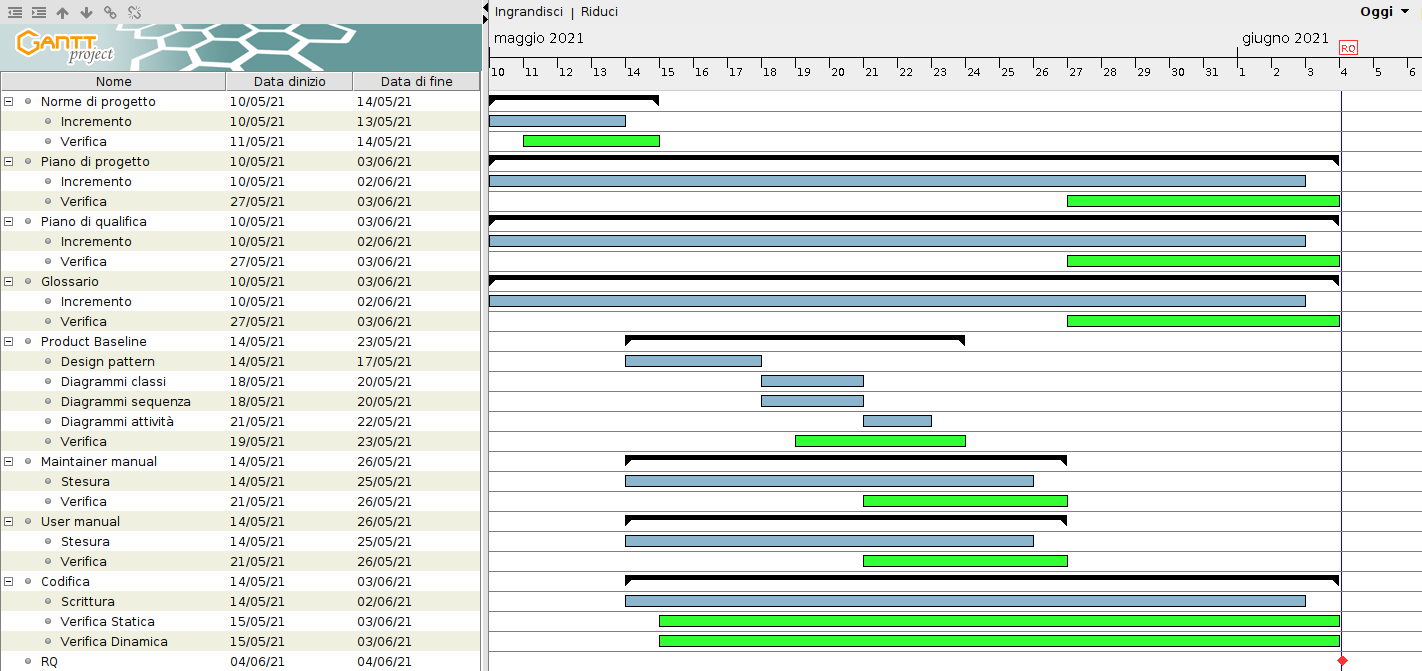
\includegraphics[scale=0.22]{../../../Images/Diagrammi/Gantt/progettazioneCodifica_v3.png}
    \centering
\end{figure}

\subsection{Validazione e collaudo}
\textit{Periodo: dal 2021-07-09 al 2021-08-23}\\
L'inizio di questa fase è il giorno della scadenza della \textit{Revisione di Qualifica} e la data di fine coincide con la data di consegna dei documenti in vista della \textit{Revisione di Accettazione}.\\
Le attività di questa fase sono:
\begin{itemize}
    \item \textbf{Incremento e verifica:} in cui i documenti precedentemente redatti vengono aggiornati e migliorati;
    \item \textbf{Validazione e collaudo:} per la parte di collaudo si eseguiranno ulteriori test sul prodotto, in modo da garantirne correttezza e stabilità. Per ciò che concerne la validazione, verrà valutata la coerenza del prodotto e dei requisiti specificati nel documento \textit{Analisi dei Requisiti} nella sua ultima versione;
\end{itemize}
Le attività di questa fase sono suddivise in quattro incrementi di sviluppo, per ognuno dei quali sono riportate le seguenti voci:
\begin{itemize}
    \item obbiettivi
          \begin{itemize}
              \item software;
              \item documentali;
          \end{itemize}
    \item periodo;
    \item ruoli attivi;
    \item attività previste;
    \item diagramma di Gantt.
\end{itemize}

%Incremento 1 RA ---------------------------------------------------------
\subsubsection{Incremento 14}
\subsubsubsection{Obbiettivi}
Gli obbiettivi che il gruppo di pone di soddisfare in questo periodo sono i seguenti:
\begin{itemize}
    \item Aggiunta ordinamento alla lista dei prodotti;
    \item Aggiunti filtri per categoria e marca;
    \item Aggiunto acquisto diretto del prodotto;;
    \item Incremento della documentazione per verifica e miglioramento continuo.
\end{itemize}
\subsubsubsection{Periodo}
Il gruppo ritiene che per il raggiungimento degli obbiettivi serviranno dieci giorni di lavoro;\\
Il periodo interessato sarà dal 2021/07/09 al 2021/07/18
\subsubsubsection{Ruoli attivi}
Il gruppo ritiene che durante questo incremento saranno attivi i seguenti ruoli:
\begin{itemize}
    \item \textit{Responsabile di progetto};
    \item \textit{Amministratore di progetto};
    \item \textit{Progettista};
    \item \textit{Programmatore};
    \item \textit{Verificatore}.
\end{itemize}
\subsubsubsection{Attività previste}
Per soddisfare gli obbiettivi preposti il gruppo ritiene di dover svolgere le seguenti attività:
\begin{itemize}
    \item implementazione del caso d'uso UC4 - Acquisto diretto del prodotto;\\requisiti:
          \begin{itemize}
              \item R5.9F.
          \end{itemize}
    \item implementazione del caso d'uso UC15 - Scelta della categoria;\\requisiti:
          \begin{itemize}
              \item R10.4F.
          \end{itemize}
    \item implementazione del caso d'uso UC34 - Ordinamento prodotti;\\requisiti:
          \begin{itemize}
              \item R9F;
              \item R9.1F;
              \item R9.2F.
          \end{itemize}
    \item implementazione del caso d'uso UC35 - Applicazione filtri;\\requisiti:
          \begin{itemize}
              \item R10.3F.
          \end{itemize}
    \item \textbf{verifica:} rilevazione delle metriche di qualità di prodotto e di processo;
    \item \textbf{ampliamento della documentazione:}
          \begin{itemize}
              \item incremento della stesura del \textit{Maintainer Manual v2.0.0} per le funzionalità complete;
              \item incremento della stesura del \textit{User Manual v2.0.0} per le funzionalità complete;
              \item aggiornamento delle metriche e degli obbiettivi di qualità per quanto concerne il prodotto software;
              \item registrazione degli esiti di verifica;
              \item registrazione dell'andamento degli obbiettivi di qualità;
              \item aggiornamento dell'analisi dei rischi e della sua attualizzazione;
              \item aggiornamento del \textit{Glossario v4.0.0};
              \item calcolo del consuntivo di periodo;
              \item calcolo del preventivo a finire rispetto alla fase;
              \item calcolo del preventivo a finire rispetto al completamento del progetto.
          \end{itemize}
\end{itemize}
\pagebreak
\subsubsubsection{Diagramma di Gantt}
\begin{figure}[!ht]
    \caption{Diagramma di Gantt dell'incremento 14}
    \vspace{5px}
    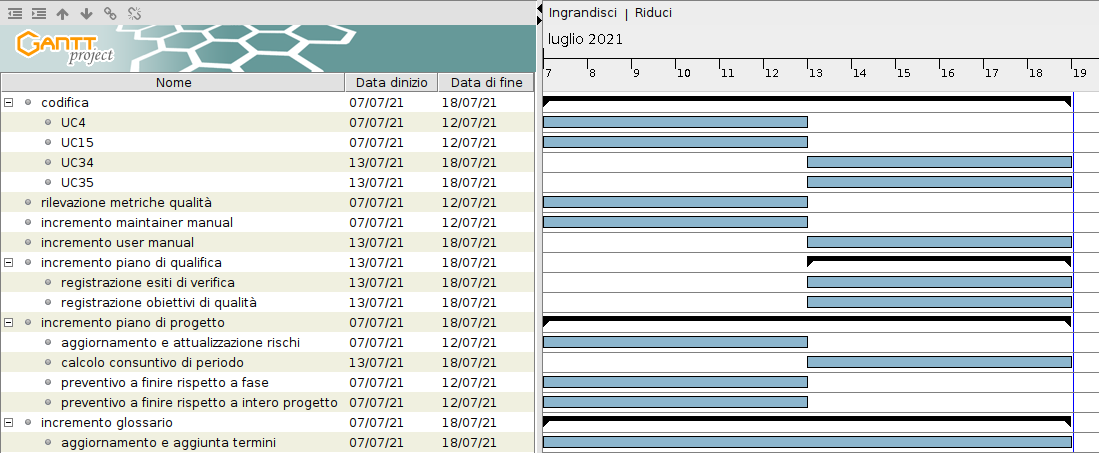
\includegraphics[scale=0.3]{../../../Images/Diagrammi/Gantt/incremento14.png}
    \centering
\end{figure}

%Incremento 2 RA ---------------------------------------------------------
\subsubsection{Incremento 15}
\subsubsubsection{Obbiettivi}
Gli obbiettivi che il gruppo di pone di soddisfare in questo periodo sono i seguenti:
\begin{itemize}
    \item Aggiunta gestione della quantità dei prodotti all'interno del carrello;
    \item Aggiunto registrazione con servizio esterno;
    \item Aggiunto autenticazione con servizio esterno;
    \item Incremento della documentazione per verifica e miglioramento continuo.
\end{itemize}
\subsubsubsection{Periodo}
Il gruppo ritiene che per il raggiungimento degli obbiettivi serviranno dodici giorni di lavoro;\\
Il periodo interessato sarà dal 2021/07/19 al 2021/07/30
\subsubsubsection{Ruoli attivi}
Il gruppo ritiene che durante questo incremento saranno attivi i seguenti ruoli:
\begin{itemize}
    \item \textit{Responsabile di progetto};
    \item \textit{Amministratore di progetto};
    \item \textit{Progettista};
    \item \textit{Programmatore};
    \item \textit{Verificatore}.
\end{itemize}
\subsubsubsection{Attività previste}
Per soddisfare gli obbiettivi preposti il gruppo ritiene di dover svolgere le seguenti attività:
\begin{itemize}
    \item implementazione del caso d'uso UC3 - Autenticazione esterna;\\requisiti:
          \begin{itemize}
              \item R4F.
          \end{itemize}
    \item implementazione del caso d'uso UC10 - Registrazione esterna;\\requisiti:
          \begin{itemize}
              \item R12F.
          \end{itemize}
    \item \textbf{analisi dei requisiti:} correzione in base alle indicazioni dei committenti ricevute in seguito alla RQ
    \item \textbf{piano di progetto:} correzione in base alle indicazioni dei committenti ricevute in seguito alla RQ
    \item \textbf{norme di progetto:} correzione in base alle indicazioni dei committenti ricevute in seguito alla RQ
    \item \textbf{piano di qualifica:} correzione in base alle indicazioni dei committenti ricevute in seguito alla RQ
    \item \textbf{verifica:} rilevazione delle metriche di qualità di prodotto e di processo;
    \item \textbf{ampliamento della documentazione:}
          \begin{itemize}
              \item incremento della stesura del \textit{Maintainer Manual v2.0.0} per le funzionalità complete;
              \item incremento della stesura del \textit{User Manual v2.0.0} per le funzionalità complete;
              \item aggiornamento delle metriche e degli obbiettivi di qualità per quanto concerne il prodotto software;
              \item registrazione degli esiti di verifica;
              \item registrazione dell'andamento degli obbiettivi di qualità;
              \item aggiornamento dell'analisi dei rischi e della sua attualizzazione;
              \item aggiornamento del \textit{Glossario v4.0.0};
              \item calcolo del consuntivo di periodo;
              \item calcolo del preventivo a finire rispetto alla fase;
              \item calcolo del preventivo a finire rispetto al completamento del progetto.
          \end{itemize}
\end{itemize}
\subsubsubsection{Diagramma di Gantt}
\begin{figure}[!ht]
    \caption{Diagramma di Gantt dell'incremento 15}
    \vspace{5px}
    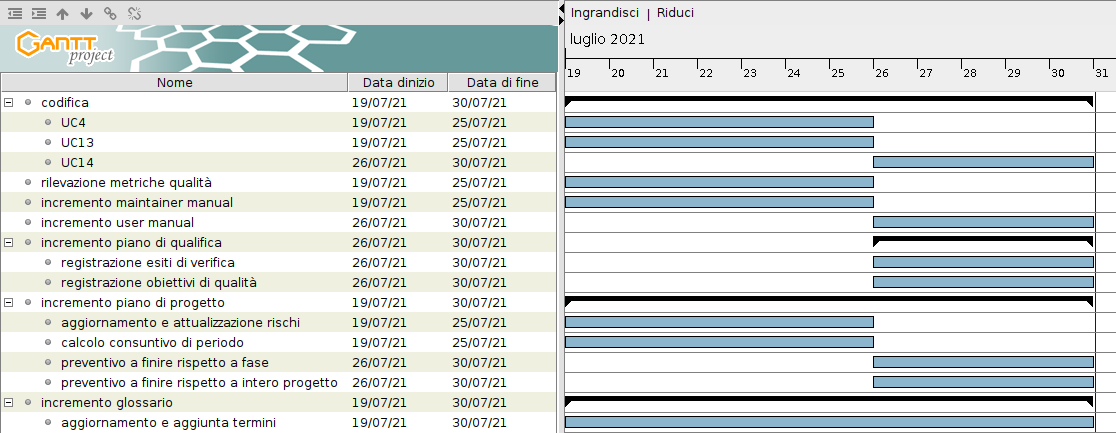
\includegraphics[scale=0.3]{../../../Images/Diagrammi/Gantt/incremento15.png}
    \centering
\end{figure}

%Incremento 3 RA ---------------------------------------------------------
\subsubsection{Incremento 16}
\subsubsubsection{Obbiettivi}
Gli obbiettivi che il gruppo di pone di soddisfare in questo periodo sono i seguenti:
\begin{itemize}
    \item Aggiunto la possibilità d'invio di messaggi tra venditore e cliente;
    \item Incremento della documentazione per verifica e miglioramento continuo.
\end{itemize}
\subsubsubsection{Periodo}
Il gruppo ritiene che per il raggiungimento degli obbiettivi serviranno diciassette giorni di lavoro;\\
Il periodo interessato sarà dal 2021/07/31 al 2021/08/16
\subsubsubsection{Ruoli attivi}
Il gruppo ritiene che durante questo incremento saranno attivi i seguenti ruoli:
\begin{itemize}
    \item \textit{Responsabile di progetto};
    \item \textit{Amministratore di progetto};
    \item \textit{Progettista};
    \item \textit{Programmatore};
    \item \textit{Verificatore}.
\end{itemize}
\subsubsubsection{Attività previste}
Per soddisfare gli obbiettivi preposti il gruppo ritiene di dover svolgere le seguenti attività:
\begin{itemize}
    \item implementazione del caso d'uso UC20 - Contatta il venditore;\\requisiti:
          \begin{itemize}
              \item R18F.
          \end{itemize}
    \item implementazione del caso d'uso UC27 - Contatta un cliente;\\requisiti:
          \begin{itemize}
              \item R25F.
          \end{itemize}
    \item \textbf{verifica:} rilevazione delle metriche di qualità di prodotto e di processo;
    \item \textbf{ampliamento della documentazione:}
          \begin{itemize}
              \item incremento della stesura del \textit{Maintainer Manual v2.0.0} per le funzionalità complete;
              \item incremento della stesura del \textit{User Manual v2.0.0} per le funzionalità complete;
              \item aggiornamento delle metriche e degli obbiettivi di qualità per quanto concerne il prodotto software;
              \item registrazione degli esiti di verifica;
              \item registrazione dell'andamento degli obbiettivi di qualità;
              \item aggiornamento dell'analisi dei rischi e della sua attualizzazione;
              \item aggiornamento del \textit{Glossario v4.0.0};
              \item calcolo del consuntivo di periodo;
              \item calcolo del preventivo a finire rispetto alla fase;
              \item calcolo del preventivo a finire rispetto al completamento del progetto.
          \end{itemize}
\end{itemize}
\pagebreak
\subsubsubsection{Diagramma di Gantt}
\begin{figure}[!ht]
    \caption{Diagramma di Gantt dell'incremento 16}
    \vspace{5px}
    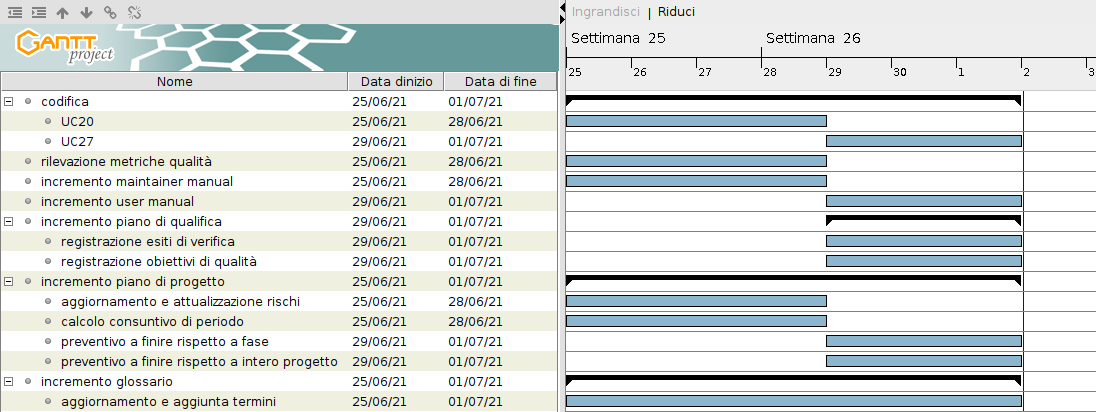
\includegraphics[scale=0.3]{../../../Images/Diagrammi/Gantt/incremento16.png}
    \centering
\end{figure}

%Incremento 4 RA ---------------------------------------------------------
\subsubsection{Incremento 17}
\subsubsubsection{Obbiettivi}
Gli obbiettivi che il gruppo di pone di soddisfare in questo periodo sono i seguenti:
\begin{itemize}
    \item Preparazione all'esposizione per la \textit{Revisione di accettazione};
    \item Preparazione per il collaudo con il proponente;
    \item Incremento della documentazione per verifica e miglioramento continuo.
\end{itemize}
\subsubsubsection{Periodo}
Il gruppo ritiene che per il raggiungimento degli obbiettivi serviranno sei giorni di lavoro;\\
Il periodo interessato sarà dal 2021/08/17 al 2021/08/22
\subsubsubsection{Ruoli attivi}
Il gruppo ritiene che durante questo incremento saranno attivi i seguenti ruoli:
\begin{itemize}
    \item \textit{Responsabile di progetto};
    \item \textit{Amministratore di progetto};
    \item \textit{Progettista};
    \item \textit{Programmatore};
    \item \textit{Verificatore}.
\end{itemize}
\subsubsubsection{Attività previste}
Per soddisfare gli obbiettivi preposti il gruppo ritiene di dover svolgere le seguenti attività:
\begin{itemize}
    \item \textbf{presentazione:} preparazione della presentazione per la \textit{Revisione di Accettazione}, e per il collaudo con il proponente;
    \item \textbf{verifica:} rilevazione delle metriche di qualità di prodotto e di processo;
    \item \textbf{ampliamento della documentazione:}
          \begin{itemize}
              \item estensione delle normative di progettazione e codifica;
              \item aggiornamento delle metriche e degli obbiettivi di qualità per quanto concerne il prodotto software;
              \item registrazione degli esiti di verifica;
              \item registrazione dell'andamento degli obbiettivi di qualità;
              \item aggiornamento dell'analisi dei rischi e della sua attualizzazione;
              \item aggiornamento del \textit{Glossario v4.0.0};
              \item calcolo del consuntivo di periodo;
              \item calcolo del preventivo a finire rispetto alla fase;
              \item calcolo del preventivo a finire rispetto al completamento del progetto.
          \end{itemize}
\end{itemize}

\subsubsubsection{Diagramma di Gantt}
\begin{figure}[!ht]
    \caption{Diagramma di Gantt dell'incremento 17}
    \vspace{5px}
    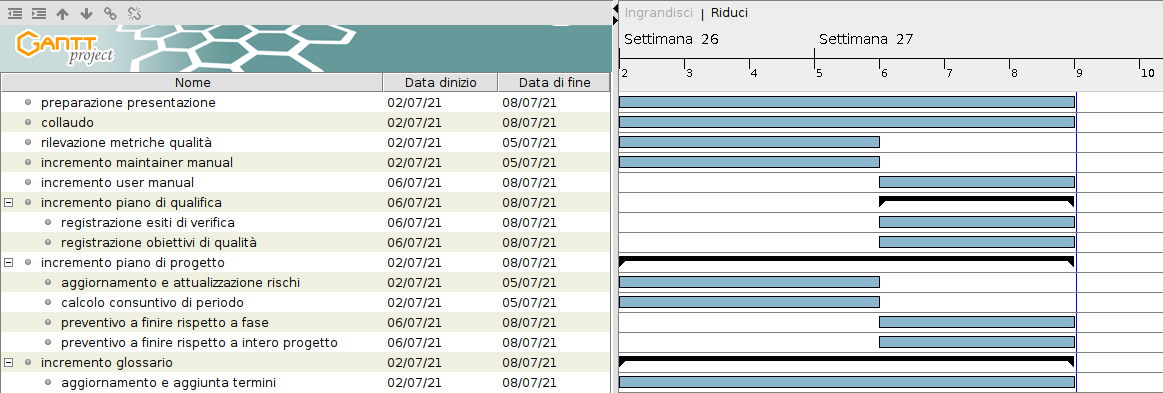
\includegraphics[scale=0.3]{../../../Images/Diagrammi/Gantt/incremento17.png}
    \centering
\end{figure}

\pagebreak
\subsubsection{Diagramma di Gantt della fase}
In base alle attività pianificate negli incrementi e alla loro distribuzione nel tempo, la pianificazione complessiva della fase può essere riassunta nel seguente diagramma.
\begin{figure}[!ht]
    \caption{Diagramma di Gantt dell'attività di Validazione e Collaudo}
    \vspace{5px}
    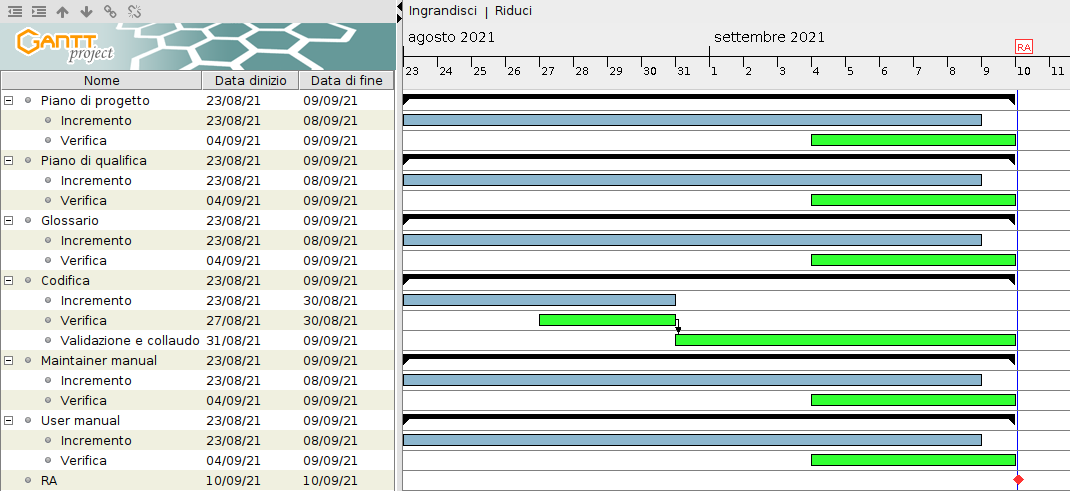
\includegraphics[scale=0.25]{../../../Images/Diagrammi/Gantt/validazione_v3.png}
    \centering
\end{figure}